\section{Análisis del Dataset y Dimensionalidad}
\label{sec:eda}

\subsection{Descripción del Dataset}
El conjunto de datos \textit{Brain Tumor Classification MRI},
publicado en Kaggle, contiene \textbf{3\,264 imágenes} de
resonancia magnética cerebral organizadas en cuatro clases
diagnósticas: \textit{glioma\_tumor}, \textit{meningioma\_tumor},
\textit{pituitary\_tumor} y \textit{no\_tumor} (estudios sin
hallazgos tumorales). Los autores del dataset proporcionan una
partición oficial entre conjuntos de entrenamiento y prueba que
se respeta en este trabajo. La Tabla~\ref{tab:dist} resume su
distribución.

\begin{table}[!t]
\centering
\caption{Distribución de imágenes por clase y partición.}
\label{tab:dist}
\begin{tabular}{lrrr}
\toprule
\textbf{Clase} & \textbf{Train} & \textbf{Test} & \textbf{Total} \\
\midrule
glioma\_tumor      & 826 & 100 & 926 \\
meningioma\_tumor  & 822 & 115 & 937 \\
no\_tumor          & 395 & 105 & 500 \\
pituitary\_tumor   & 827 &  74 & 901 \\
\midrule
\textbf{Total}     & \textbf{2\,870} & \textbf{394} & \textbf{3\,264} \\
\bottomrule
\end{tabular}
\end{table}

El conjunto de entrenamiento concentra el \textbf{87{,}9\,\%}
de las imágenes (2\,870), mientras que el conjunto de prueba
representa el \textbf{12{,}1\,\%} restante (394 imágenes). El
conjunto \textit{Testing} se reserva como \textit{holdout}
independiente para la evaluación final de los modelos, y la
subdivisión interna para validación se realiza únicamente sobre
\textit{Training} (véase Sección~\ref{sec:proto}).

\subsection{Balance de Clases}
El análisis de balance evidencia que la clase \textit{no\_tumor}
es la minoritaria en entrenamiento, con aproximadamente
\textbf{395} imágenes, frente a $\sim$\textbf{825} para cada una
de las tres clases tumorales. Esta proporción asimétrica
($\sim$1:2) puede inducir sesgos durante el aprendizaje, llevando
al modelo a sub-representar la clase minoritaria y a inflar
artificialmente la \textit{Accuracy} global.

Como estrategia de compensación se adopta el uso de pesos por
clase (\textit{class\_weight}) en la función de pérdida
\textit{Cross-Entropy}, con ponderaciones inversamente
proporcionales a la frecuencia relativa de cada clase en el
conjunto de entrenamiento. Esto incrementa la magnitud del
gradiente para errores cometidos sobre la clase minoritaria sin
alterar la distribución de muestras observadas. Las
Figuras~\ref{fig:balance} y \ref{fig:pie} ilustran gráficamente
esta distribución.

\begin{figure}[!t]
\centering
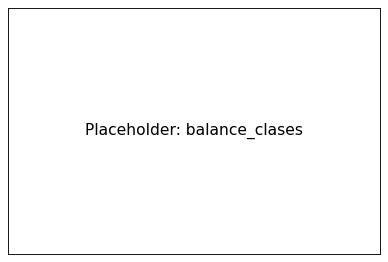
\includegraphics[width=\columnwidth]{../../outputs/figures/balance_clases.png}
\caption{Distribución absoluta por clase y partición.}
\label{fig:balance}
\end{figure}

\begin{figure}[!t]
\centering
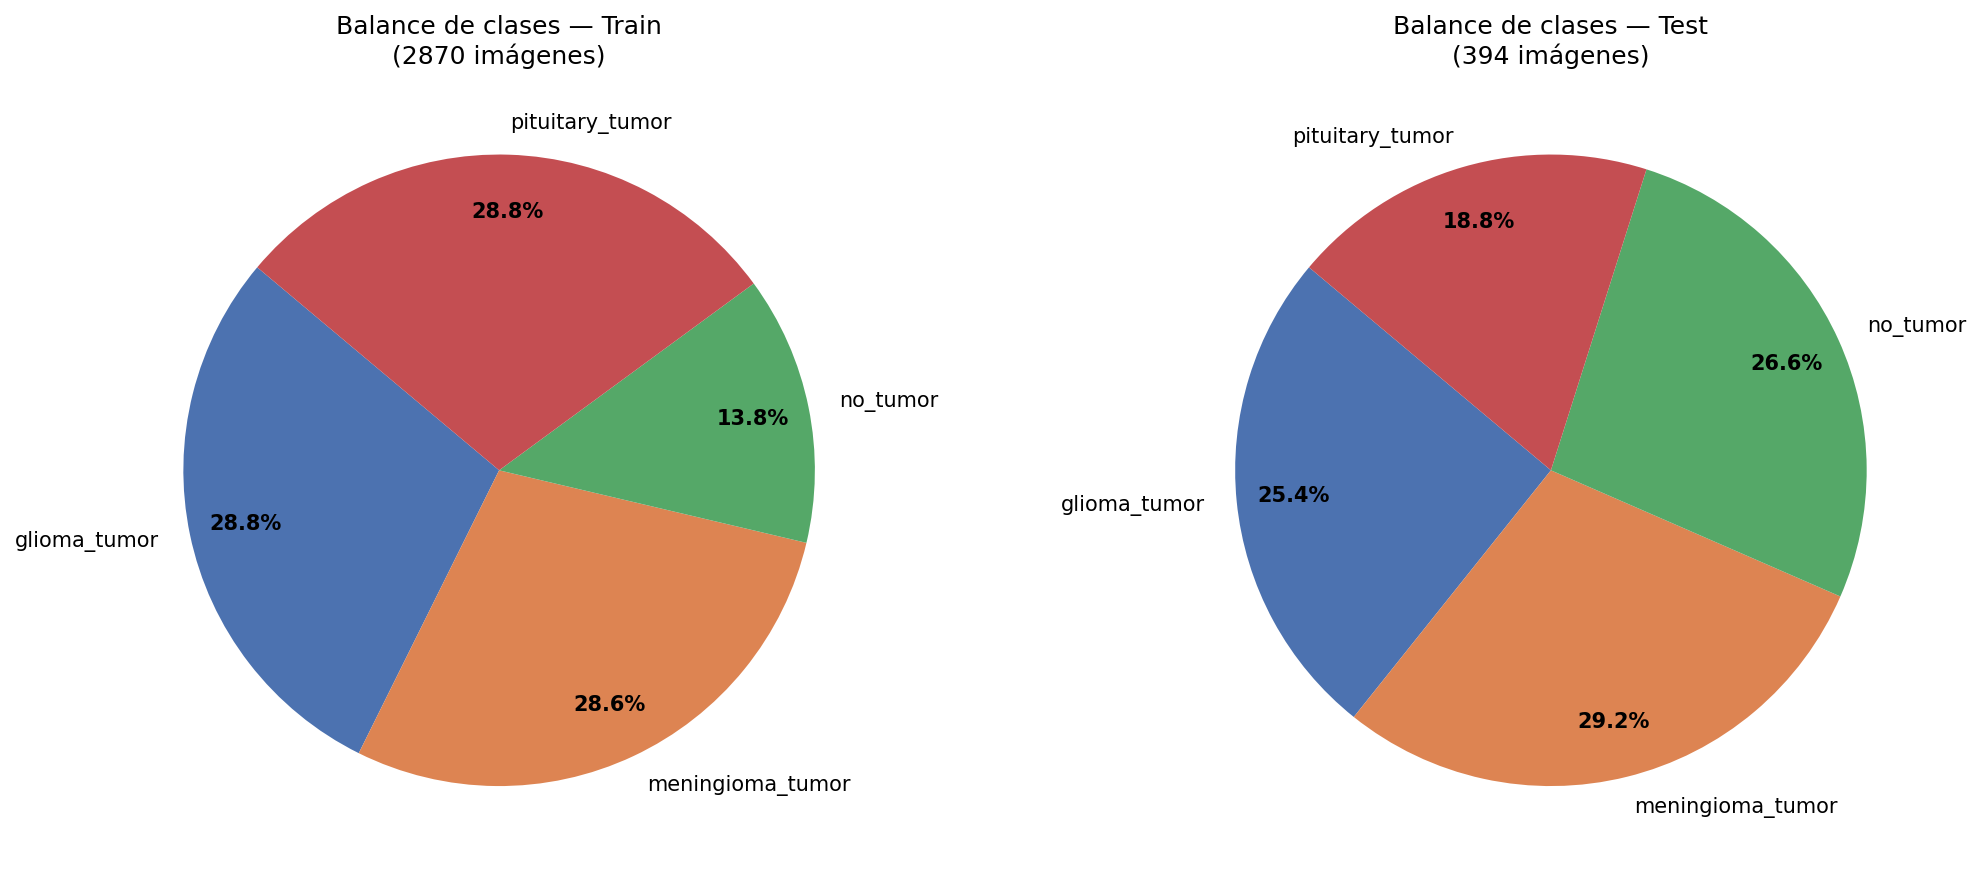
\includegraphics[width=0.75\columnwidth]{../../outputs/figures/pie_balance.png}
\caption{Proporción relativa en entrenamiento.}
\label{fig:pie}
\end{figure}

\subsection{Análisis de Dimensionalidad}
Se inspeccionó una muestra de \textbf{80 imágenes por clase}
para caracterizar la variabilidad en resolución espacial del
dataset. Las imágenes presentan resoluciones altamente
heterogéneas: las dimensiones máximas observadas alcanzan
\textbf{1024$\times$768\,px} y las mínimas \textbf{59$\times$80\,px}.
La relación de aspecto también varía considerablemente entre
estudios, reflejo de las diferencias entre equipos de adquisición
y protocolos clínicos.

Dada esta heterogeneidad, se establece el redimensionamiento
uniforme a \textbf{224$\times$224\,px} como paso obligatorio del
pipeline. Esta resolución constituye un compromiso adecuado
entre el nivel de detalle anatómico preservado y el costo
computacional, y es además el formato canónico de las
arquitecturas CNN modernas, lo que facilita comparaciones
posteriores. Las Figuras~\ref{fig:hist-res} y \ref{fig:aspect}
muestran respectivamente el histograma de resoluciones y la
distribución de relaciones de aspecto observadas por clase.

\begin{figure}[!t]
\centering
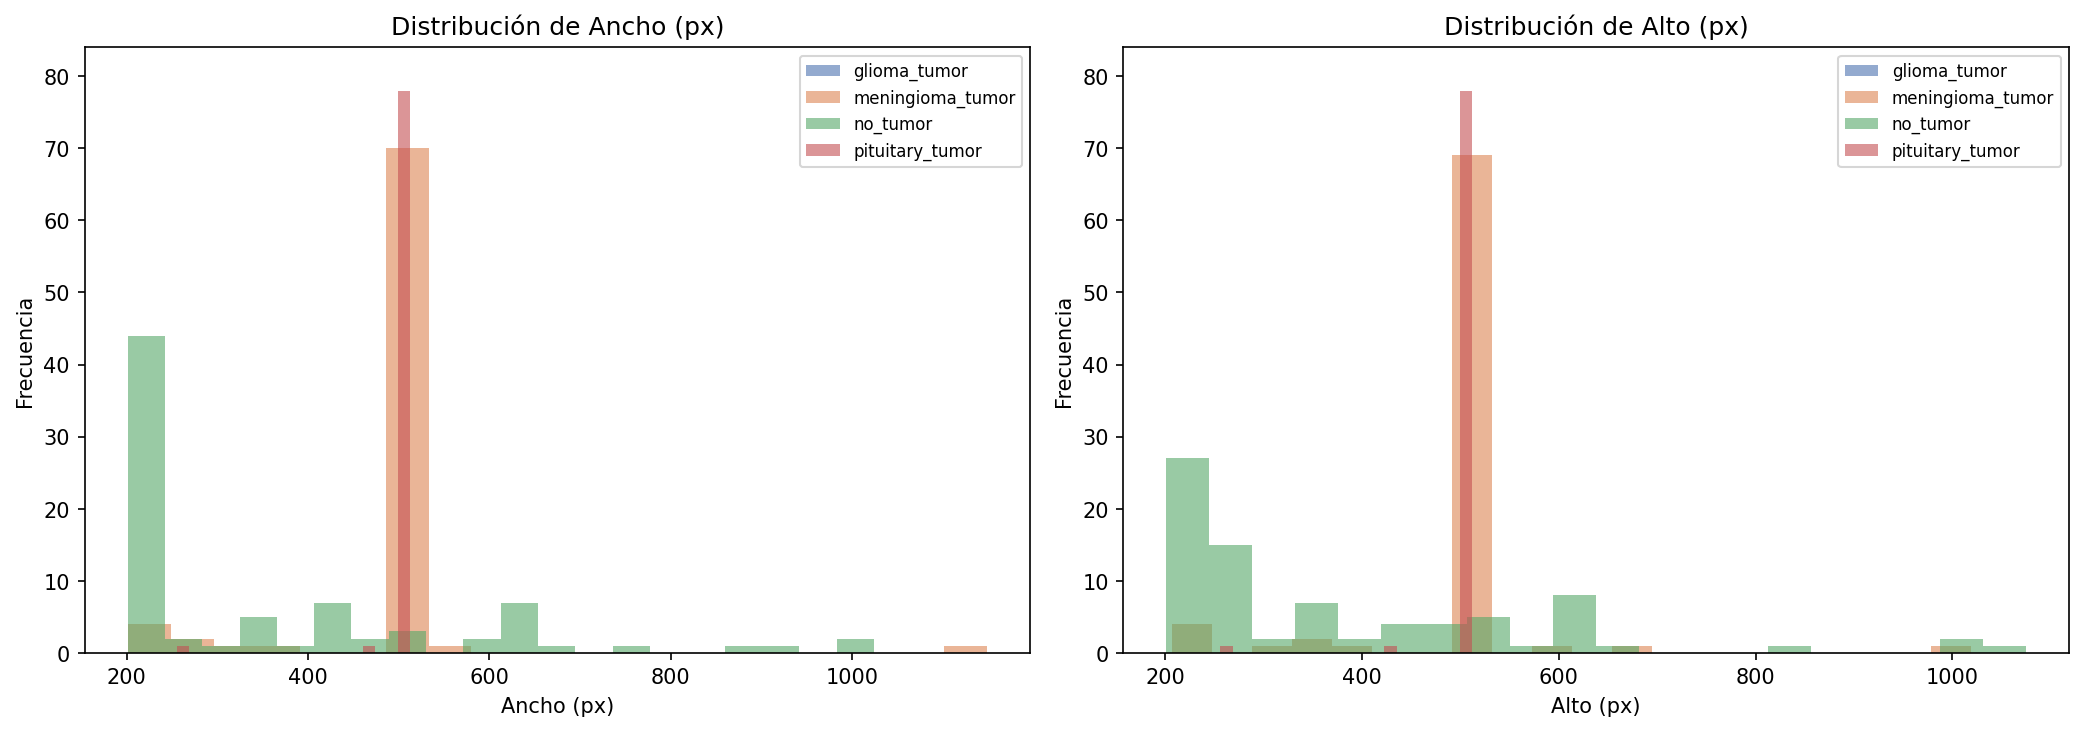
\includegraphics[width=\columnwidth]{../../outputs/figures/histograma_resolucion.png}
\caption{Histograma de resoluciones (ancho $\times$ alto) en el
dataset.}
\label{fig:hist-res}
\end{figure}

\begin{figure}[!t]
\centering
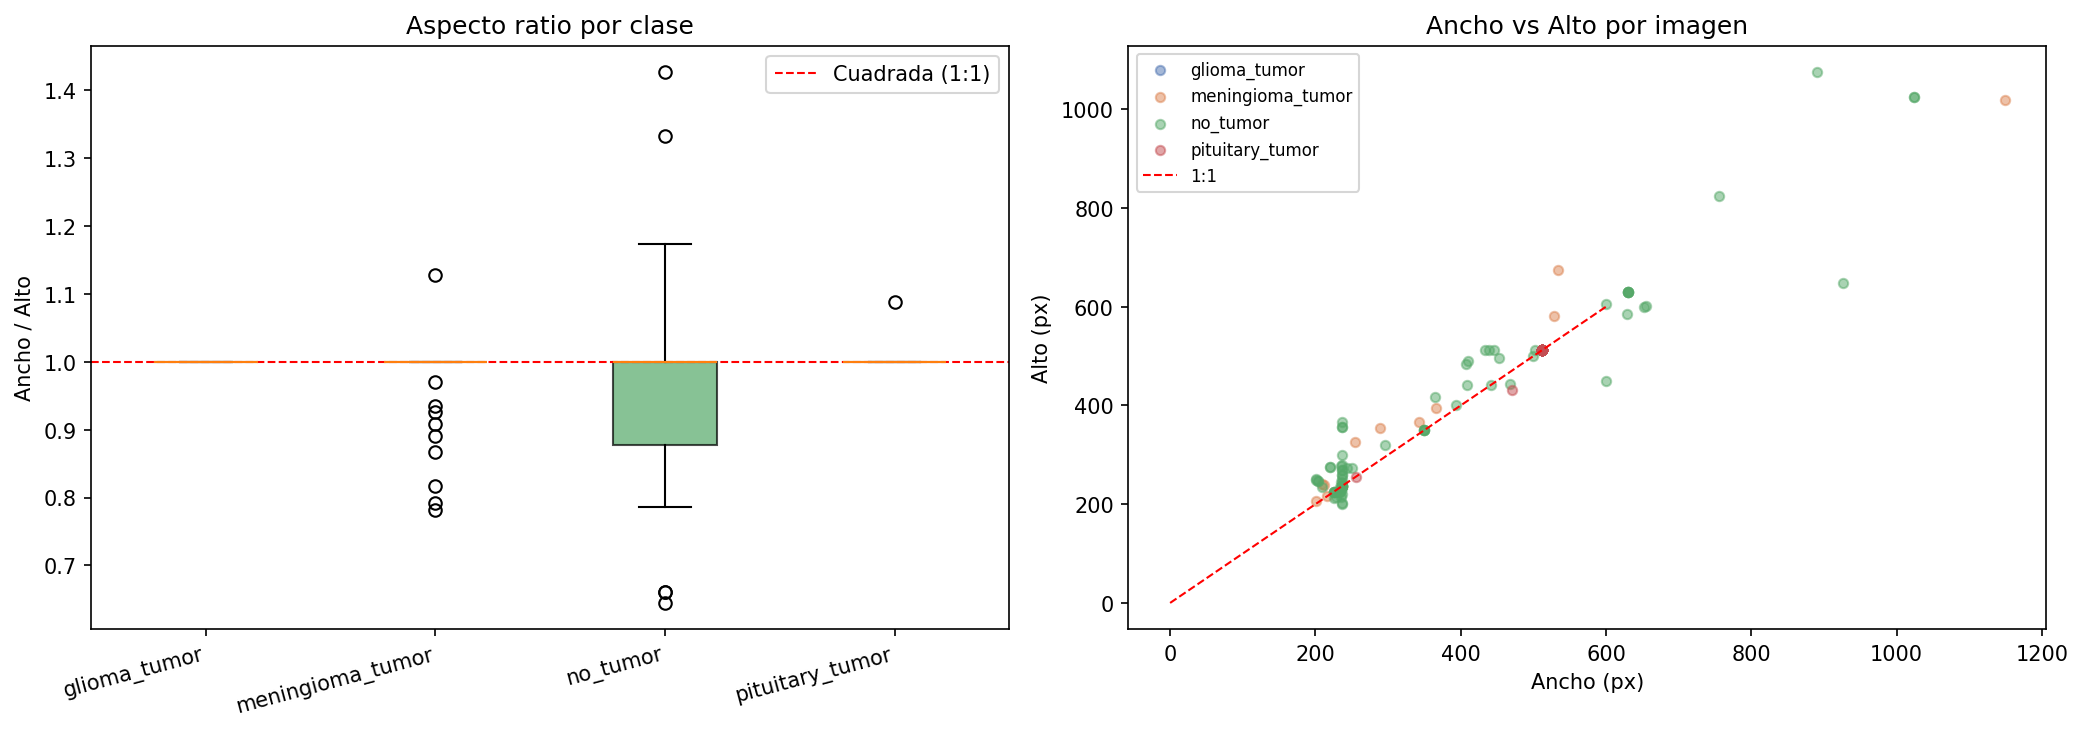
\includegraphics[width=\columnwidth]{../../outputs/figures/aspecto_ratio.png}
\caption{Distribución de relaciones de aspecto por clase.}
\label{fig:aspect}
\end{figure}

\subsection{Análisis Estadístico de Intensidades}
Se analizaron las distribuciones de intensidad de píxeles
(escala de grises) y canales RGB por clase, con el fin de
identificar diferencias fotométricas potencialmente
discriminativas para el modelado. La Tabla~\ref{tab:stats}
resume los estadísticos descriptivos.

\begin{table}[!t]
\centering
\caption{Estadísticas de intensidad (escala 0--255) por clase.}
\label{tab:stats}
\begin{tabular}{lrrrrr}
\toprule
\textbf{Clase} & \textbf{Media} & \textbf{Std} & \textbf{Mín} & \textbf{Máx} & \textbf{Mediana} \\
\midrule
glioma\_tumor     & 36{,}23 & 41{,}43 & 0 & 255 & 14 \\
meningioma\_tumor & 44{,}56 & 47{,}77 & 0 & 255 & 28 \\
no\_tumor         & 52{,}21 & 59{,}63 & 0 & 255 & 22 \\
pituitary\_tumor  & 49{,}50 & 42{,}94 & 0 & 255 & 50 \\
\bottomrule
\end{tabular}
\end{table}

Los \textit{gliomas} presentan los valores más bajos de media
(36{,}23) y mediana (14), lo que los caracteriza como tejidos
relativamente \textbf{hipointensos} en la modalidad analizada.
Los tumores \textit{pituitarios}, en contraste, presentan la
mediana más alta (50) y la menor dispersión relativa, indicando
intensidades más concentradas y homogéneas. La clase
\textit{no\_tumor} muestra la mayor desviación estándar
(59{,}63), consistente con la variedad anatómica del cerebro
sano sin focalización lesional. Estas diferencias fotométricas
constituyen señales útiles que una CNN puede explotar a nivel
de filtros convolucionales de bajo nivel.

Para estabilizar el entrenamiento se aplicará normalización
\textit{Z-score} sobre los tres canales utilizando los
estadísticos canónicos de ImageNet ($\mu = [0{,}485, 0{,}456,
0{,}406]$, $\sigma = [0{,}229, 0{,}224, 0{,}225]$), valores
ampliamente adoptados en la literatura como referencia robusta
incluso cuando no se emplea \textit{transfer learning}. Las
Figuras~\ref{fig:box} y \ref{fig:rgb} complementan visualmente
este análisis.

\begin{figure}[!t]
\centering
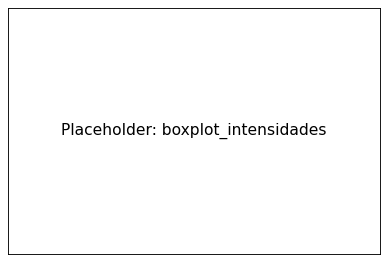
\includegraphics[width=\columnwidth]{../../outputs/figures/boxplot_intensidades.png}
\caption{Diagramas de caja de intensidades de píxel por clase.}
\label{fig:box}
\end{figure}

\begin{figure}[!t]
\centering
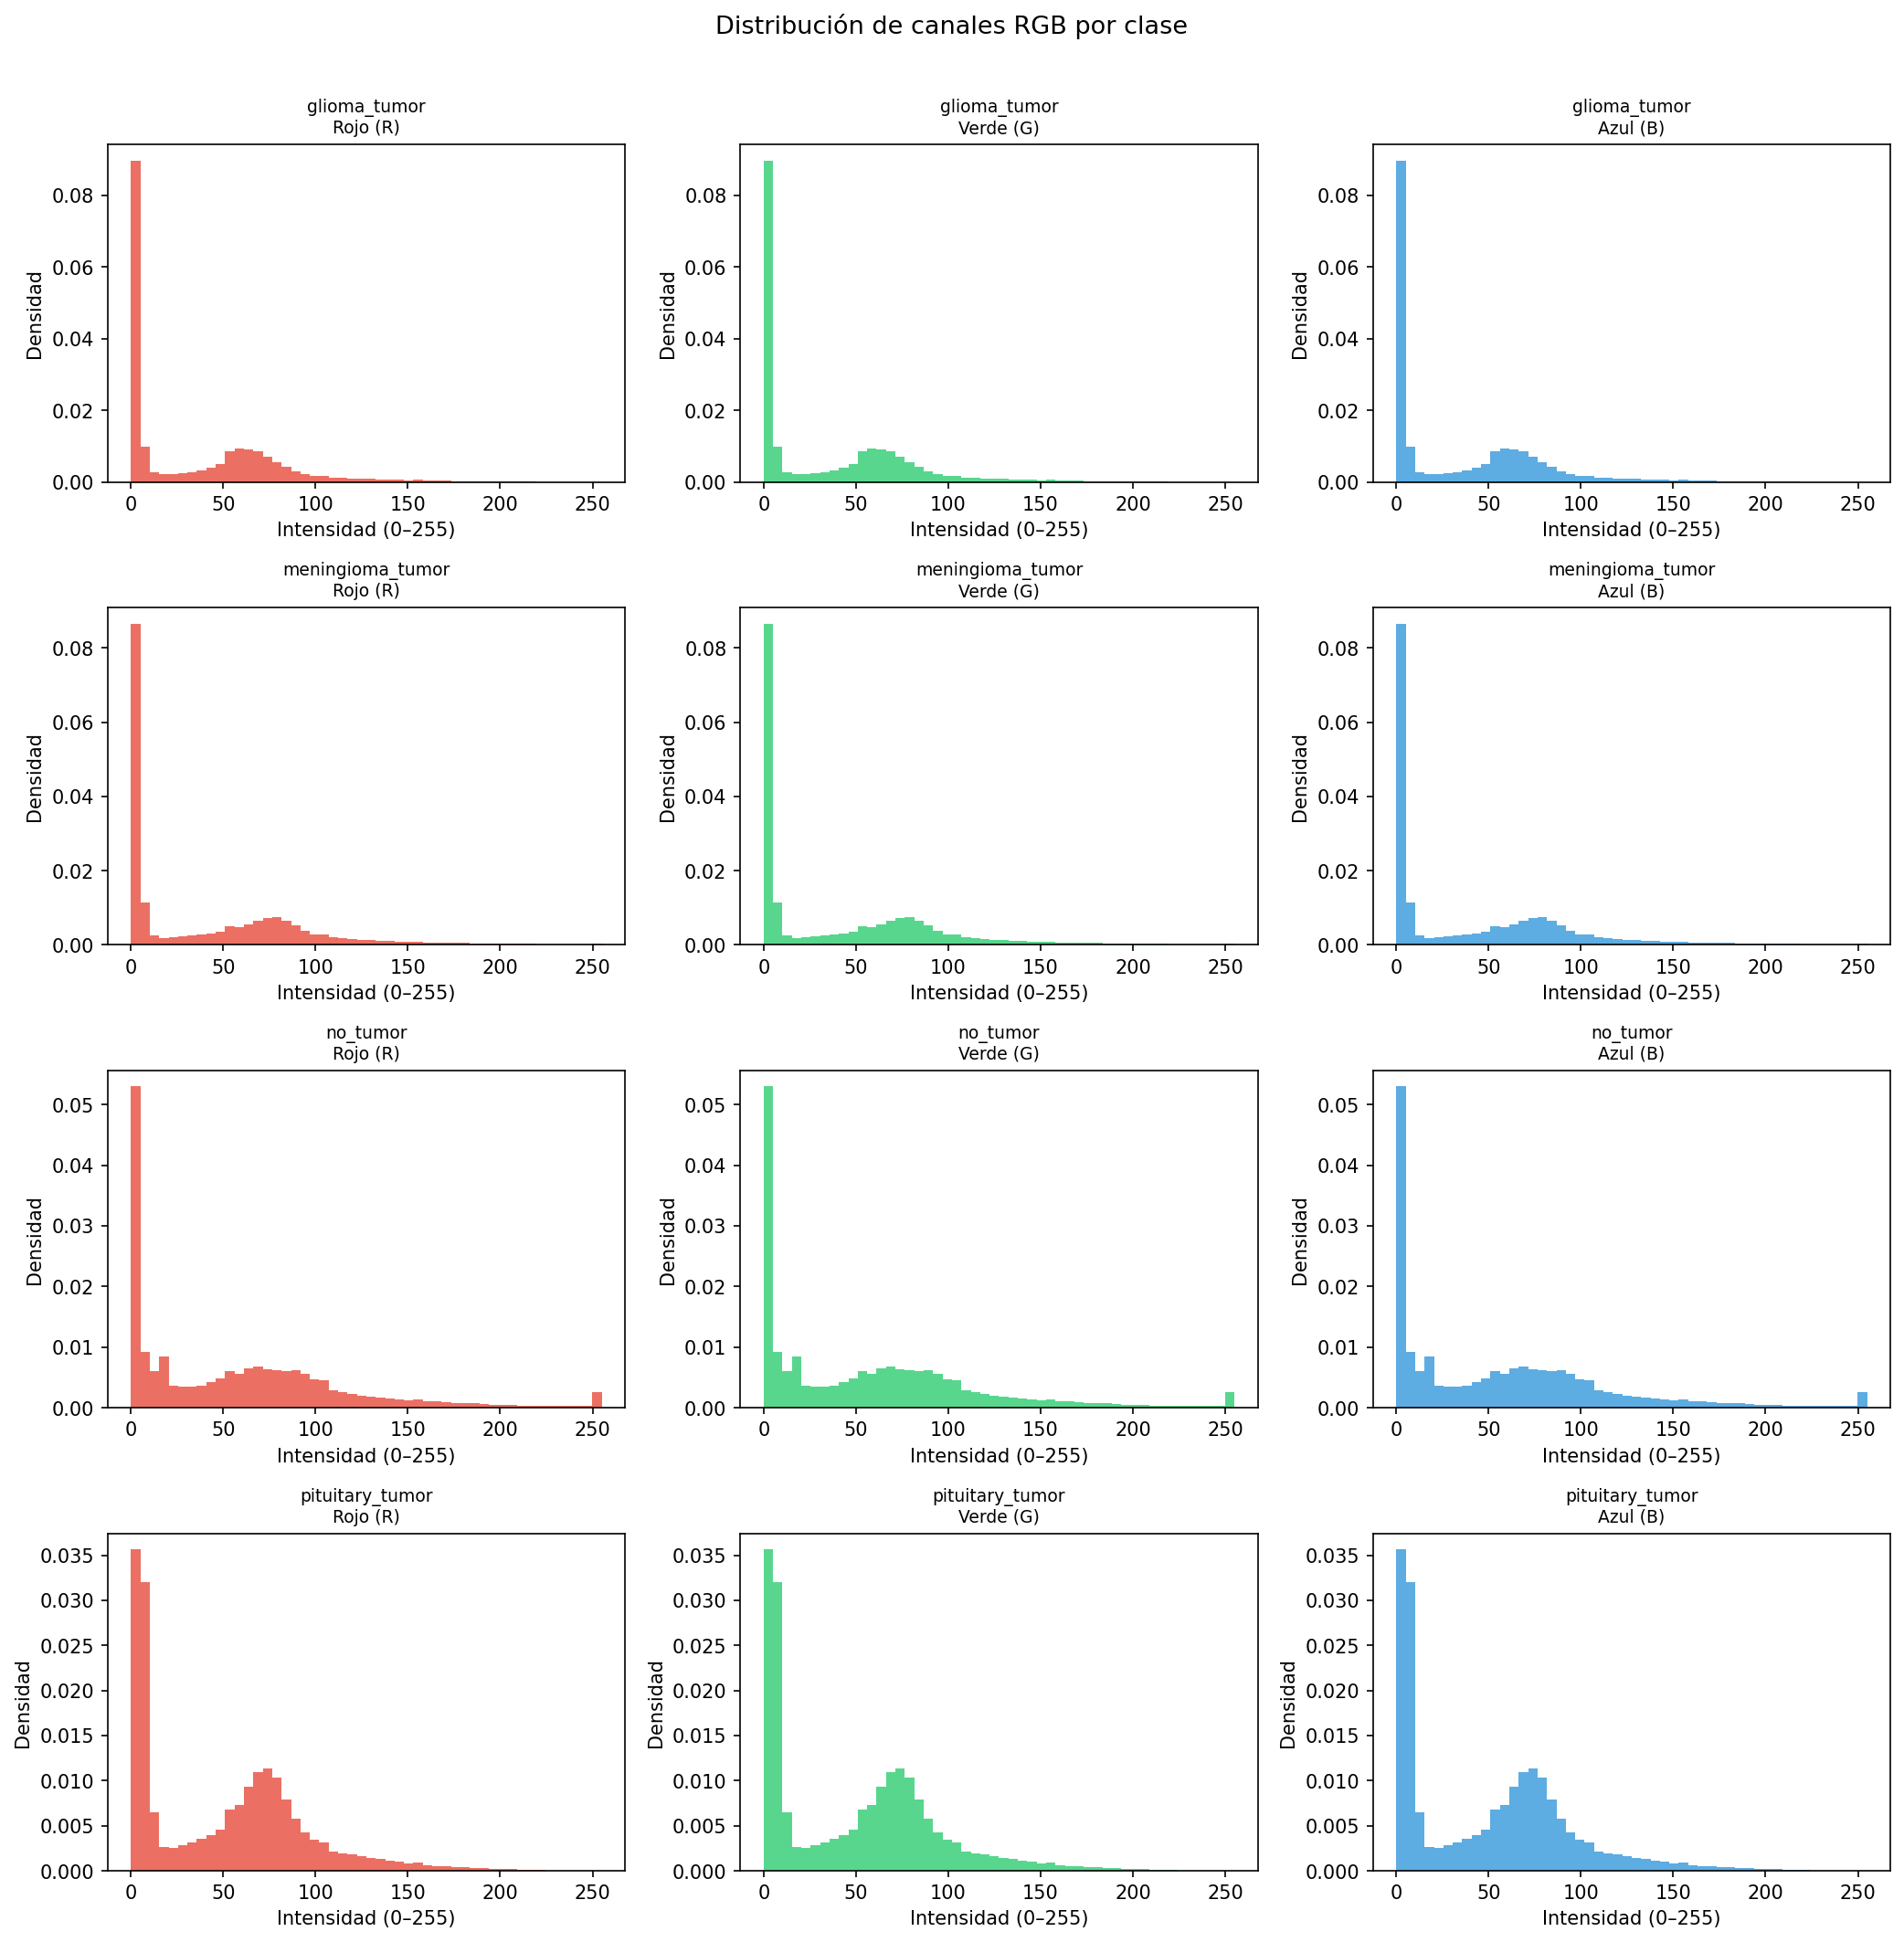
\includegraphics[width=\columnwidth]{../../outputs/figures/canales_rgb.png}
\caption{Distribución de intensidades por canal RGB y por
clase.}
\label{fig:rgb}
\end{figure}

\subsection{Imagen Promedio y Muestras por Clase}
La Figura~\ref{fig:promedio} presenta la imagen promedio por
clase, calculada como la media píxel a píxel de 100 imágenes
redimensionadas a 224$\times$224\,px. Los gliomas exhiben
regiones \textbf{hipointensas difusas}, de bordes poco
definidos, consistente con su naturaleza infiltrativa. Los
tumores \textit{pituitarios} tienden a concentrarse en la zona
central, reflejando la ubicación anatómica de la glándula
hipófisis. Los meningiomas muestran patrones intermedios con
tendencia a localizarse en la periferia. La clase
\textit{no\_tumor}, al promediar tejidos cerebrales sanos en
distintas orientaciones, produce una imagen más difusa y
centralmente simétrica.

\begin{figure}[!t]
\centering
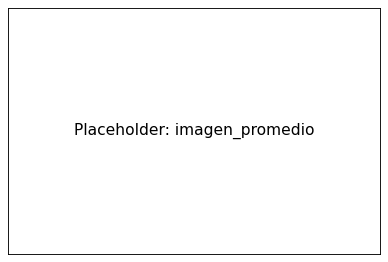
\includegraphics[width=\columnwidth]{../../outputs/figures/imagen_promedio.png}
\caption{Imagen promedio por clase (100 imgs, 224$\times$224
px).}
\label{fig:promedio}
\end{figure}

La Figura~\ref{fig:muestras} ilustra cinco ejemplos
representativos por clase. Se evidencia alta variabilidad
intra-clase en orientación, escala y contraste, lo que justifica
el uso de \textit{data augmentation} ---rotación
$\pm 15^{\circ}$, \textit{flip} horizontal y variación de
brillo--- durante el entrenamiento para mejorar la capacidad de
generalización del modelo.

\begin{figure}[!t]
\centering
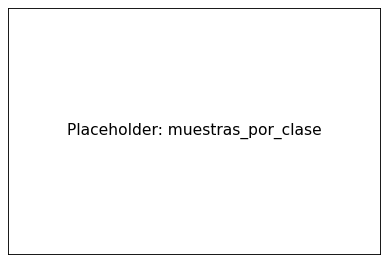
\includegraphics[width=\columnwidth]{../../outputs/figures/muestras_por_clase.png}
\caption{5 muestras por clase --- \textit{Training}.}
\label{fig:muestras}
\end{figure}

\subsection{Plan de Preprocesamiento}
A partir de los hallazgos anteriores, se define el pipeline de
preprocesamiento resumido en la Tabla~\ref{tab:pipe}, aplicado
de forma consistente a las tres arquitecturas evaluadas.

\begin{table}[!t]
\centering
\caption{Pipeline de preprocesamiento propuesto.}
\label{tab:pipe}
\begin{tabularx}{\columnwidth}{clX}
\toprule
\textbf{\#} & \textbf{Paso} & \textbf{Justificación} \\
\midrule
1 & Resize 224$\times$224\,px & Resoluciones heterogéneas requieren entrada uniforme. \\
2 & Conversión a RGB           & Algunas imágenes en escala de grises; se unifica formato. \\
3 & Z-score ($\mu$ ImageNet)   & Estabiliza el gradiente y mejora la convergencia. \\
4 & \textit{Data augmentation} & Rotación $\pm 15^{\circ}$, \textit{flip} horizontal y variación de brillo. \\
5 & \textit{class\_weight}     & Compensa el desbalance de \textit{no\_tumor}. \\
6 & Split 80/20 \textit{Training} & Separa validación sin contaminar el \textit{holdout} oficial. \\
\bottomrule
\end{tabularx}
\end{table}
